\ifx\mainfile\undefined
%  ========================================================================
%  Copyright (c) 2006-2011 The University of Washington
%
%  Licensed under the Apache License, Version 2.0 (the "License");
%  you may not use this file except in compliance with the License.
%  You may obtain a copy of the License at
%
%      http://www.apache.org/licenses/LICENSE-2.0
%
%  Unless required by applicable law or agreed to in writing, software
%  distributed under the License is distributed on an "AS IS" BASIS,
%  WITHOUT WARRANTIES OR CONDITIONS OF ANY KIND, either express or implied.
%  See the License for the specific language governing permissions and
%  limitations under the License.
%  ========================================================================
%
 
\documentclass [11pt, twoside] {uwthesis}

\usepackage{color}
\usepackage{url}
\usepackage{amsmath}
\usepackage{amsfonts}
\usepackage[bookmarks,
	hidelinks,
	plainpages=false,
	pdfpagelabels,
	pagebackref=true,
            ]{hyperref}
\renewcommand*{\backref}[1]{}% for backref < 1.33 necessary
\renewcommand*{\backrefalt}[4]{%
  \ifcase #1 %
    (No citations.)%
  \or
    (Cited on page #2.)%
  \else
    (Cited on pages #2.)%
  \fi
}

\newcommand{\biburl}[1]{{\tt<}\url{#1}{\tt>}}

\hypersetup{%
pdfauthor = {Daniel Chaim Halperin},
pdftitle = {Simplifying the Configuration of 802.11 Wireless Networks with Effective SNR},
pdfsubject = {Ph.D. Dissertation},
pdfkeywords = {},
pdfcreator = {University of Washington, Computer Science and Engineering},
pdfproducer = {},
bookmarksopen = {true},
pdfpagelayout = {TwoColumnRight},
}

\usepackage{footnotebackref}
%%%%%%%%%%%%%%%%%%%%%%%%%%%%%%%%%%%%%%%%%%%%%%%%%%%%%%
%%%        Formatting sections                     %%%
%%%%%%%%%%%%%%%%%%%%%%%%%%%%%%%%%%%%%%%%%%%%%%%%%%%%%%
\newcommand{\algref}[1]{Algorithm~\ref{#1}}
\newcommand{\chapref}[1]{Chapter~\ref{#1}}
\renewcommand{\eqref}[1]{Equation~\ref{#1}}
\newcommand{\figref}[1]{Figure~\ref{#1}}
\newcommand{\secref}[1]{\S\ref{#1}}
\newcommand{\tabref}[1]{Table~\ref{#1}}
\newcommand{\heading}[1]{\vspace{4pt}\noindent\textbf{#1}}
\newcommand{\topheading}[1]{\noindent\textbf{#1}}
\newcommand{\noheading}[0]{\vspace{4pt}\noindent}

%%%%%%%%%%%%%%%%%%%%%%%%%%%%%%%%%%%%%%%%%%%%%%%%%%%%%%
%%%        XXX and other warnings                  %%%
%%%%%%%%%%%%%%%%%%%%%%%%%%%%%%%%%%%%%%%%%%%%%%%%%%%%%%
\newcommand{\xxx}[1]{\textit{\color{red}XXX #1}}

%%%%%%%%%%%%%%%%%%%%%%%%%%%%%%%%%%%%%%%%%%%%%%%%%%%%%%
%%%        Units                                   %%%
%%%%%%%%%%%%%%%%%%%%%%%%%%%%%%%%%%%%%%%%%%%%%%%%%%%%%%
\usepackage{xspace}
\newcommand{\unitsep}{\texorpdfstring{\,}{ }}
\def\unit#1{% from: http://www.tex.ac.uk/cgi-bin/texfaq2html?label=csname "Defining a macro from an argument"
  \expandafter\def\csname #1\endcsname{\unitsep\text{#1}\xspace}%
}
\def\varunit#1#2{% from: http://www.tex.ac.uk/cgi-bin/texfaq2html?label=csname "Defining a macro from an argument"
  \expandafter\def\csname #1\endcsname{\unitsep\text{#2}\xspace}%
}
\unit{GHz}
\unit{MHz}
\unit{kHz}
\unit{Gbps}
\unit{Mbps}
\unit{KB}
\unit{dB}
\unit{dBi}
\unit{dBm}
\unit{W}
\unit{mW}
\varunit{uW}{$\mu$W}
\unit{ms}
\varunit{us}{$\mu$s}
\unit{h}
\unit{m}
\unit{s}
\unit{km}
\unit{cm}
\unit{mm}
\varunit{mmsq}{mm$^\text{2}$}
\varunit{insq}{in$^\text{2}$}
\newcommand{\degree}{\ensuremath{^\circ}\xspace}
\newcommand{\degrees}{\degree}
%%%%%%%%%%%%%%%%%%%%%%%%%%%%%%%%%%%%%%%%%%%%%%%%%%%%%%%%%%%%%%%%%%%%%%%%%%%%%%%%%%%%%%
% Euler for math | Palatino for rm | Helvetica for ss | Courier for tt
%
% From: http://www.tug.org/mactex/fonts/LaTeX_Preamble-Font_Choices.html
%%%%%%%%%%%%%%%%%%%%%%%%%%%%%%%%%%%%%%%%%%%%%%%%%%%%%%%%%%%%%%%%%%%%%%%%%%%%%%%%%%%%%%
\renewcommand{\rmdefault}{ppl} % rm
\usepackage[scaled]{helvet} % ss
\usepackage{courier} % tt
\usepackage{eulervm} % a better implementation of the euler package (not in gwTeX)
\normalfont
\usepackage[T1]{fontenc}
%%%%%%%%%%%%%%%%%%%%%%%%%%%%%%%%%%%%%%%%%%%%%%%%%%%%%%%%%%%%%%%%%%%%%%%%%%%%%%%%%%%%%%

%%%%%%%%%%%%%%%%%%%%%%%%%%%%%%%%%%%%%%%%%%%%%%%%%%%%%%
%%%        Figures                                 %%%
%%%%%%%%%%%%%%%%%%%%%%%%%%%%%%%%%%%%%%%%%%%%%%%%%%%%%%
\usepackage{graphicx}
% Caption package both lets you set the spacing between figure and caption
% and also makes the \figref{} point to the right place.
\usepackage[font=bf,aboveskip=6pt,belowskip=-4mm]{caption}
% Allow subfigures, make them bold
\usepackage[bf,BF,small]{subfigure}
% List of figures
\setcounter{lofdepth}{2}  % Print the chapter and sections to the lot

%%%%%%%%%%%%%%%%%%%%%%%%%%%%%%%%%%%%%%%%%%%%%%%%%%%%%%
%%%        Lists with reduced spacing              %%%
%%%%%%%%%%%%%%%%%%%%%%%%%%%%%%%%%%%%%%%%%%%%%%%%%%%%%%
\usepackage{enumitem}

%%%%%%%%%%%%%%%%%%%%%%%%%%%%%%%%%%%%%%%%%%%%%%%%%%%%%%
%%%        Fancy tables                            %%%
%%%%%%%%%%%%%%%%%%%%%%%%%%%%%%%%%%%%%%%%%%%%%%%%%%%%%%
\usepackage{tabulary}
\usepackage{booktabs}

%%%%%%%%%%%%%%%%%%%%%%%%%%%%%%%%%%%%%%%%%%%%%%%%%%%%%%
%%%        Formatting techniques/tools/etc.        %%%
%%%%%%%%%%%%%%%%%%%%%%%%%%%%%%%%%%%%%%%%%%%%%%%%%%%%%%
\newcommand{\term}[1]{\texttt{#1}}

\begin{document}
 
\textpages
\setcounter{chapter}{1} % Set to n-1!
\fi
%%%%%%%%%%%%%%%%%%%%%%%%%%%%%%%%%%

\cleardoublepage
\chapter{Background}
\label{chap:background}

In this chapter, I establish the fundamentals of wireless communication and the IEEE 802.11 standards to the extent needed to understand my thesis.

\section{Digital Communication Principles}
Electromagnetic (EM) communications, which send data using \define{electromagnetic signals}, form the basis of the technologies I will discuss in this thesis. One key aspect of each technology is which part of the electromagnetic spectrum it uses, characterized by its \define{carrier frequency or center frequency}, denoted $f_c$. IEEE~802.11 networks typically use EM signals with a carrier frequency in the range of 2.4\GHz and 5\GHz.

Data transmission using EM signals works by \define{modulating} a pure sine wave with frequency $f_c$, i.e.\ by transforming the sine wave to reflect the underlying data. The simplest modulation scheme might be to turn the sine wave on or off depending on whether the bit to be transmitted is a 1 or a 0. The rate at which the signal changes---in this example, the rate the sine wave is turned on or off---is called the \define{baud rate or symbol rate}, and determines the \emph{bandwidth} of the channel $B$ measured in Hertz (Hz).

In a \define{link}, that is a sender communicating data to a receiver, the sender generates a signal with \define{transmit (signal) power} level $T$ that propagates through the \define{channel} connecting the two. The channel could be a \define{wire} or it could be the free-space \define{radio frequency (RF)} environment in which signals propagate from the transmitter's antenna to the receiver's antenna over the air.

\subsection{The wired channel}
To simplify the discussion, I will start with the case of a wired channel. The transmitted signal propagates down the wire to the receiver and then is received with \define{receive (signal) power} $S$, which I will also refer to as its \define{amplitude}. While propagating through the wire, the signal gets slightly weaker as a small amount of energy is absorbed. This effect is called \define{attenuation}, denoted $\alpha$, and is defined mathematically as the multiplicative decrease in power induced by the channel:
\begin{equation}
	\label{eq:attenuation}
	\alpha = \frac{T}{S}.
\end{equation}
In addition to attenuation, the wired channel also induces a \define{phase shift} as the electromagnetic signal propagates. The value of this phase shift, denoted $\theta$, depends on factors including the length of the wire and the frequency of the signal, and is generally considered to be an unknown, uniformly random quantity between $0$ and $2\pi$.

The signal measured by the receiver is also corrupted by broad-spectrum electromagnetic noise. This corruption is sometimes called \define{Johnson-Nyquist noise} after its identification in 1927 by Johnson~\cite{Johnson_noise} and explanation in 1928 by Nyquist~\cite{Nyquist_noise}, but is more commonly known as \define{thermal noise}. Thermal noise is modeled as a complex Gaussian with average \define{noise power} $N$ (in Watts) equal to
\begin{equation}
\label{eq:noise}
N = kTB,
\end{equation}
where $k\approx1.38\times10^{-23}$ (in Joules/kelvin) is Boltzmann's constant, $T$ is the temperature (in kelvins), and $B$ is the bandwidth as described above. This model is also called additive, white Gaussian noise (AWGN).
%For a device at room temperature ($\approx$ 293\K), we can compute $N$ in dBm using the approximation
%\begin{equation}
%N \text{ (dBm)} = -174 + 10\log_{10}(B).
%\end{equation}

In the context of 802.11, we typically measure power-related quantities on a logarithmic scale to capture the wide range of possible values. Power levels such as the quantities $T$, $S$, and $N$ are usually measured in decibels relative to 1~milliwatt, or dBm, and typically take on values like $T=20\dBm$ and $S=-80\dBm$. To calculate $N$, we can use \eqref{eq:noise}: Wi-Fi links typically use bandwidths $B$ of 20\MHz or 40\MHz, which correspond to thermal noise levels of $-$101\dBm and $-$98\dBm at room temperature. In practice, we also assume a 10\dB--15\dB \define{noise figure}, a quantity that estimates additional noise added by imperfect analog hardware used in receiver processing.

Now that we have defined the signal and noise powers, we can discuss the limits of the communication channel. The seminal works of Ralph Hartley~\cite{Hartley_law} and Claude Shannon~\cite{Shannon_coding,Shannon_capacity} proved that the \define{capacity} of a channel---i.e., the maximum data rate $R$ at which the transmitter and receiver can communicate---is determined by the channel's bandwidth ($B$ as above) and its \define{signal-to-noise ratio (SNR\@)}. The SNR\@, denoted by $\rho$, is a unitless quantity typically measured in decibels and calculated as
\begin{equation}
\rho = \frac{S}{N}.
\end{equation}
The Shannon-Hartley Theorem~\cite{Shannon_capacity} establishes what is called the \define{Shannon capacity} to be
\begin{equation}
\label{eq:shannon_capacity}
R = B\log(1+\rho).
\end{equation}
\figref{fig:shannon} shows this relationship for the normalized quantity $R/B$.

\begin{figure}[htb]
\centering
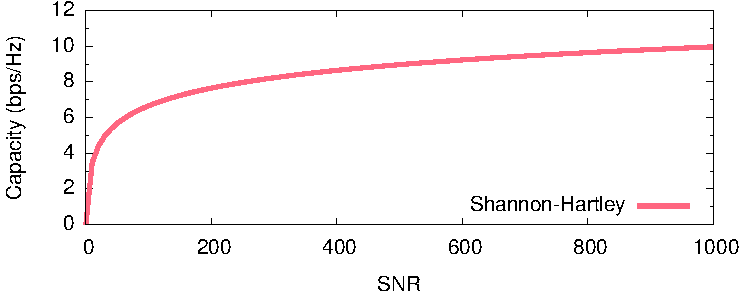
\includegraphics{calculations/shannon-crop}
\caption{\label{fig:shannon}The Shannon Capacity of a communications channel with Gaussian noise.}
\end{figure}

The Shannon-Hartley Theorem determines a bound on the maximum rate achievable as a function of the bandwidth and signal strength. However, it does not give a practical scheme that realizes this bound, and instead systems like 802.11 use a set of many different schemes that achieve different points along the curve, and choose among these in practice depending on the underlying channel conditions.

The binary modulation system I discussed above is a scheme called On-Off Keying~(OOK\@). Each symbol conveys 1 bit, and since the symbol rate is directly tied to the bandwidth used by a scheme, OOK can deliver at most 1 bps/Hz. A generalized form of OOK is Amplitude Shift Keying~(ASK\@), which can send more bits per symbol using multiple power levels. $m$-ASK, i.e., ASK with $m$ power levels per symbol, can deliver up to $\log_2(m)$ bits per symbol and thus can achieve a higher capacity.

\begin{figure}[t]
\centering
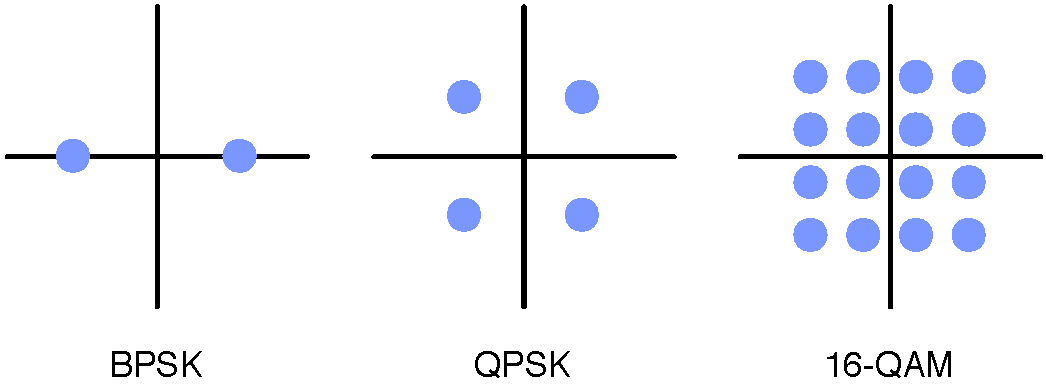
\includegraphics[width=0.8\textwidth]{figures/constellations}
\caption{\label{fig:constellations}Constellation diagrams for the BPSK, QPSK, and 16-QAM modulations.}
\end{figure}

As mentioned above, electromagnetic signals actually have both an amplitude and a phase. Amplitude modulation varies one of these parameters, and a complementary scheme called Phase-Shift Keying~(PSK) keeps the amplitude constant but varies the phase. A third scheme known as Quadrature Amplitude Modulation~(QAM) varies both parameters simultaneously and results in a more efficient system when sending more than 2 bits per symbol. Noting that the polar coordinates given by amplitude and phase can equivalently be thought of as a complex number, $m$-QAM can be equivalently thought of as $\sqrt{m}$-ASK in both the real and complex dimensions simultaneously. \figref{fig:constellations} shows the two-dimensional \define{constellations} that result from picturing the symbols sent in BPSK (i.e.\ 2-PSK), QPSK (i.e.\ 4-PSK), and 16-QAM modulation schemes.

There are many more modulation schemes than I have presented here, but PSK and QAM are the modulations applicable to 802.11.
%Currently, Wi-Fi devices transmit data using 2-PSK (called Binary PSK, or BPSK), 4-PSK (called Quadrature PSK\@, or QPSK\@), 16-QAM\@, or 64-QAM\@.
64-QAM is the highest modulation currently used by Wi-Fi devices, though the future IEEE 802.11ac amendment~\cite{80211ac} will add 256-QAM to this set.

\begin{figure}[ht]
\centering
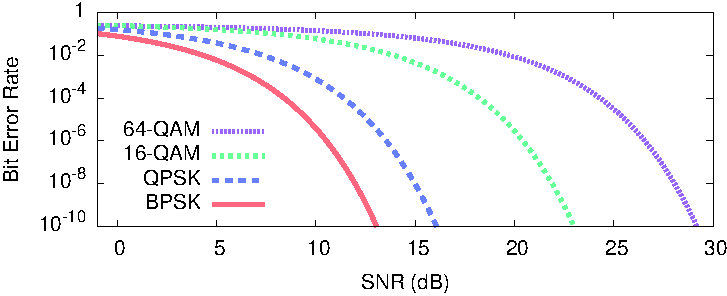
\includegraphics{calculations/snr_ber-crop}
\caption{\label{fig:mod_ber_snr}The relationship between bit error rate and SNR for the four 802.11 modulation schemes.}
\end{figure}

I have not yet mentioned the disadvantage of using higher modulation schemes like 64-QAM\@. When a transmitter uses a modulation scheme that carries more bits per symbol, each bit receives a smaller faction of the total transmitted power and hence is more susceptible to noise. This effect is visible intuitively in the constellation diagrams of \figref{fig:constellations}. If the noise is thought of as shifting the received signal along a random vector in the complex space, then it a shorter vector (lower noise power) is required to cause an error by shifting the received signal from near the correct symbol to close to a different constellation point. \figref{fig:mod_ber_snr} illustrates the magnitude of this effect for the modulations used by 802.11 using textbook formulas~\cite{Sklar} that relate the SNR to a bit error rate.

\begin{figure}[t]
\centering
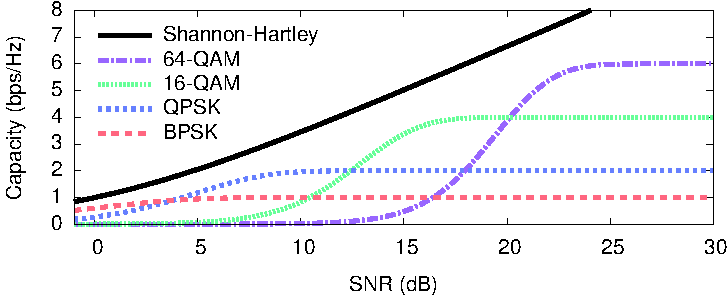
\includegraphics{calculations/snr_bits-crop}
\caption{\label{fig:mod_bits_snr}The relationship between SNR and capacity for standard modulation schemes and idealized codes.}
\end{figure}

Finally, we can now connect these different modulations back to the Shannon-Hartley Capacity Theorem by examining the capacity achieved by each scheme as a function of SNR (\figref{fig:mod_bits_snr}). In this graph, I assume an idealized coding scheme that delivers the maximum data rate for a given bit error rate; the practical schemes in widespread use today are somewhat less efficient.\footnote{Though beyond the scope of this thesis, a number of recent proposals for practical \define{rateless codes}~\cite{Gudipati_Strider,Perry_Spinal} nearly achieve the Shannon Capacity bound by using much denser constellations and clever coding schemes.}

\subsection{The wireless channel}
The previous section explained the basics of digital communications in the context of a wired link. Here, I expand to the significantly more complex case of a wireless channel.

In a wireless link, the electromagnetic signal is emitted from an antenna as a \define{radio wave} that then radiates through the \define{wireless medium}, i.e.\ the environment. The dominant source of attenuation in an wireless link is not absorption by the medium, but instead is the three-dimensional spread of energy throughout the environment, of which a small fraction is captured by a receiver's antenna. This effect, called \define{path loss}, and is captured by the Friis transmission equation:
\begin{equation}
\label{eq:friis}
	S \propto \frac{T}{d^n},
\end{equation}
where $d$ is the distance between transmitter and receiver, and $n$ is the path loss exponent. In a vacuum, $n$ would taken on a value of 2, reflecting the fact that the energy transmitted at a particular time is spread out over the surface of a sphere (or a different geometric shape in the case of a directional antenna). The path loss exponent varies in different indoor environments, but empirically tends to take on a value between 2 and 4~\cite{Sklar}.

There are many other important wireless channel effects---such as \define{shadowing}, in which materials such as glass or metal prevent radio waves from passing through---but the most problematic effect for indoor wireless links like those used in Wi-Fi is \define{multi-path fading}. At 2.4\GHz and 5\GHz, RF signals bounce off metal and glass surfaces that are common indoors. This scattering leads to a situation in which many copies of the signal arrive at the receiver having traveled along many different paths. When these copies combine, they may add constructively, giving a good overall signal, or destructively, mostly canceling the overall signal, all depending on the relative phases of the different copies. Measurement studies of fading report signal variations as high as 15--20\dB~\cite{Judd_CHARM}; I will also present experimental evidence confirming these effects in the environments I studied in \chapref{chap:problem}.

In the presence of multi-path fading, small changes in path lengths can alter the situation from good to bad because the wavelengths at 2.4\GHz and 5\GHz (the distance over which the RF signals go through a complete phase) are only 12\cm and 6\cm. Statistical models tell us that multi-path fading effects are independent for locations separated by as little as half a wavelength. This means that multi-path causes rapid signal changes or fast fading as the receiver moves, or in the case of a stationary node as the surrounding environment changes. Because multi-path effects depend on the phases of signals, they are strongly \define{frequency selective}. This means that some unlucky frequencies in a wide channel may be wiped out while others are unaffected. I will present an example in the next chapter.

The net effect of multi-path fading is that the received wireless signal can vary significantly over time, frequency and space. This is a problem for good performance because at any given time there is a significant probability of a deep fade that will reduce the SNR of the channel below the level needed for a given communication scheme.

For a variety of practical reasons, but in large part to combat multi-path fading, many modern protocols use Orthogonal Frequency Division Multiplexing (OFDM), in which a wide frequency band is split into many \define{subcarriers} that each carry different modulated bits in parallel.
%In 802.11, the 20\MHz-wide channel is broken into 64 \define{subcarriers}, each using 312.5\kHz of bandwidth.
%The beauty of OFDM is that it divides the channel in a way that is both computationally and spectrally efficient. High aggregate data rates can be achieved, while the encoding and decoding on different subcarriers can use shared hardware components.
The individual subcarriers yield relatively independently faded channels (because of multi-path fading), and hence provide \define{frequency diversity} that is realized by coding across them.

Dividing the channel also increases the symbol time per channel, since many slow symbols are sent in parallel instead of many fast symbols in sequence. This adds \define{time diversity} because the channel is more likely to average out fades over a longer period of time. Additionally, OFDM links compensate for multi-path by repeating each symbol for a short \define{guard interval} that creates a period of time in which the secondary copies of the prior symbol can arrive, and the \define{inter-symbol} overlap can be ignored by the receiver.
%In 802.11, which is targeted for roughly 100\m links, a secondary path might travel 200\m before reflecting, delayed by 667\ns from a pure line-of-sight path; 802.11 uses an 800\ns guard interval to compensate.  


\begin{itemize}
\item Multi-antenna techniques improve reliability and increase capacity in a number of ways. More transmit/receive antennas means better reliability through spatial diversity. More spatial streams means more capacity via spatial multiplexing. Together these are what we call MIMO techniques.

\item Fading, multipath, Doppler, etc. All of the above describe how we can get capacity out of the wireless channel. The hard part, and what most of all Wi-Fi research centers around, is how we develop protocols and systems to realize this capacity in the face of these effects.

\item Collisions and SINR.

\end{itemize}


\section{The IEEE 802.11n standard}
\begin{itemize}
\item IEEE 802.11 standard group offers wireless local area network connectivity. Targeted at low power ($<$1\W), medium range ($\approx$100\m) connections.
\item Unlicensed spectrum in ISM and other bands. Necessitates decentralized protocols.
\item Physical layer uses modulations, coding, OFDM, MIMO as described above. Specific base 20\MHz, single-stream configurations and the resulting data rates are shown in \tabref{tab:siso_mcs}. One key aspect is that 802.11 mandates that all data be modulated and coded identically.
\item The 802.11n enhancements are shown in \tabref{tab:11n_enhancements}. Most of improvement in the maximum data rate comes from the ability to use wider channels and multiple spatial streams. Together, these add $2\cdot2\cdot4=16$ times as many configurations to the space of a single link. Beamforming is effectively an analog parameter and adds nearly unbounded options.\footnote{For transmitter and receiver each using 4 antennas on a 40\MHz channel, representing the beamforming matrices at maximal resolution takes 29,184 bits.}
\item Hardware/software interface. Packets\footnote{We mostly ignore batching in this thesis.} are sent to the hardware and transmitted over the air. Receiver detects them from energy, estimates channel coefficients from the preamble, and then decodes the packet. Standard behavior is that all bits must be correct in order to receive the packet. Sends correct packet, plus physical layer metrics to the software stack.

\item RSSI was included in the 802.11 standard as ``a measure by the [physical layer hardware] of the energy observed at the antenna used to receive the current [packet].'' There are no specified requirements on its accuracy, instead, it is only required to be ``a monotonically increasing function of the received power''~\cite[\S 17.2.3.2]{80211}, and is generally used by the hardware to tell whether another device is transmitting. According to the standards makers, one of the intended purposes of the RSSI is ``to aid in link optimization algorithms such as roaming decisions''~\cite[\S 19.9.5.10]{80211}.
\end{itemize}

\begin{table}[t]
\centering
%\footnotesize
\begin{tabular}{cccc}
\toprule
\bf MCS & \bf Modulation & \bf Coding Rate & \bf Data Rate (Mbps) \\
\midrule
0 & BPSK & 1/2 & 6.5 \\
1 & QPSK & 1/2 & 13.0\\
2 & QPSK & 3/4 & 19.5\\
3 & 16-QAM & 1/2 & 26.0\\
4 & 16-QAM & 3/4 & 39.0\\
5 & 64-QAM & 2/3 & 52.0\\
6 & 64-QAM & 3/4 & 58.5\\
7 & 64-QAM & 5/6 & 65.0\\
\bottomrule
\end{tabular}
\caption[The 802.11n single-stream rates.]{\label{tab:siso_mcs} The single-stream 802.11n modulation and coding schemes. The first seven rates correspond to 802.11a/g rates (excluding 9\Mbps) with four added OFDM subcarriers; the highest data rate uses a new 5/6-rate code. The data rates are given for 20\MHz channels with 4\ms symbols.}
\end{table}

\begin{table}[t]
\centering
%\footnotesize
\begin{tabular}{ccc}
\toprule
\bf Enhancement & \bf Gain & \bf Description \\
\midrule
Short OFDM & \multirow{2}{*}{$1.11\times$} & Data can be more efficiently encoded\\
Guard Interval & & when the multi path delay spread is low.\\
\multirow{2}{*}{Spatial Multiplexing} & \multirow{2}{*}{$2\times$ to $4\times$} & \multirow{2}{*}{Up to 4 concurrent spatial streams.} \\
\\
Wider 40\MHz & \multirow{2}{*}{$2.08\times$} & \multirow{2}{*}{More bandwidth, higher capacity (\eqref{eq:shannon_capacity}).} \\
Channels\\
\multirow{3}{*}{Beamforming} & \multirow{3}{*}{??} & A sender with multiple transmit antennas \\
& &  can shape its signal to match the RF channel, \\
& & improving both performance and reliability. \\
\bottomrule
\end{tabular}
\caption[The 802.11n physical layer enhancements.]{\label{tab:11n_enhancements} IEEE~802.11n adds a number of enhancements to the base single-stream configurations depicted in \tabref{tab:siso_mcs}.}
\end{table}

%%%%%%%%%%%%%%%%%%%%%%%%%%%%%%%%%%
\ifx\mainfile\undefined
%
% ==========   Bibliography   ==========
%
%\nocite{*}   % include everything in the uwthesis.bib file
\bibliographystyle{plain}
\bibliography{dhalperi_thesis}

\end{document}
\fi
